\section{Reconstruction and Scalability of Coordinate Descent}
%\textbf{Coordinate Descent comparison to CLEAN reconstruction}
In this section, we compare the Coordinate Descent reconstruction with CLEAN on simulated MeerKAT data, and compare the runtime complexity of the two approaches on a real-world MeerKAT observation. We show that Coordinate Descent reconstructs the image by only computing a few columns of the Fourier Transform Matrix $F^{-1}$, and investigate if this approach reduces the runtime complexity on the large scale reconstruction problems of MeerKAT.

The real world MeerKAT data were calibrated and averaged down to reduce its size to 88 Gigabytes. The raw, uncalibrated data ranges between 500 and 1000 Gigabytes. Data on this scale requires a mature pipeline for reading and image reconstruction. Within the time limit of this project, only a reconstruction with the WSCLEAN\cite{offringa2014wsclean} pipeline was possible.

The simulations were created with the Meqtrees software package. Two simulations which contain roughly (size of Visibilities) perfectly calibrated Visibilities were created. Compared to real-world observations, the two simulated data sets are small and not representative of the real data volume. Also, more realistic simulations which contain pointing errors, calibration errors, and thermal noise are out of scope for this project. The simulations are used to isolate the two fundamental issues in radio interferometer image reconstruction: Non-uniform sampling and incomplete measurements.

\subsection{Imaging on Simulated Data}
Two simulations were created, one with two point sources shown in figure \ref{results:point}, and the other in figure \ref{results:mixed} with three gaussian extended emissions plus 16 point sources. The Coordinate Descent algorithm was compared to the CASA tCLEAN implementation. CASA is an established software framework for radio interferometer image reconstruction and was already used in a previous project.

\begin{figure}[h]
	\centering
	\begin{subfigure}[b]{0.4\linewidth}
		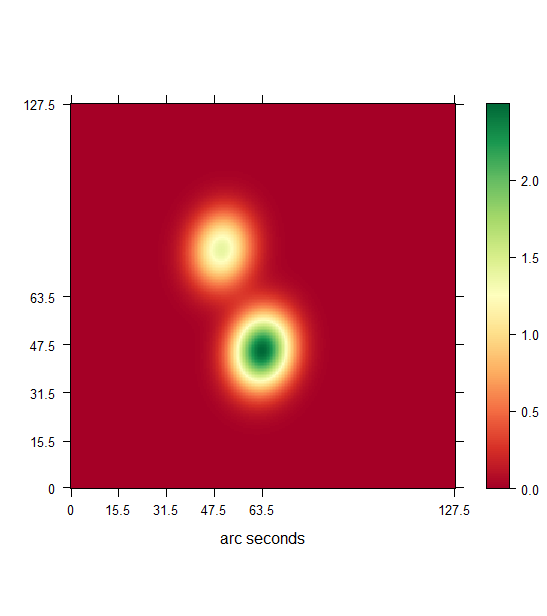
\includegraphics[width=\linewidth]{./chapters/20.results/points/tCLEAN.png}
		\caption{tCLEAN reconstruction.}
		\label{results:points:tclean}
	\end{subfigure}
	\begin{subfigure}[b]{0.4\linewidth}
		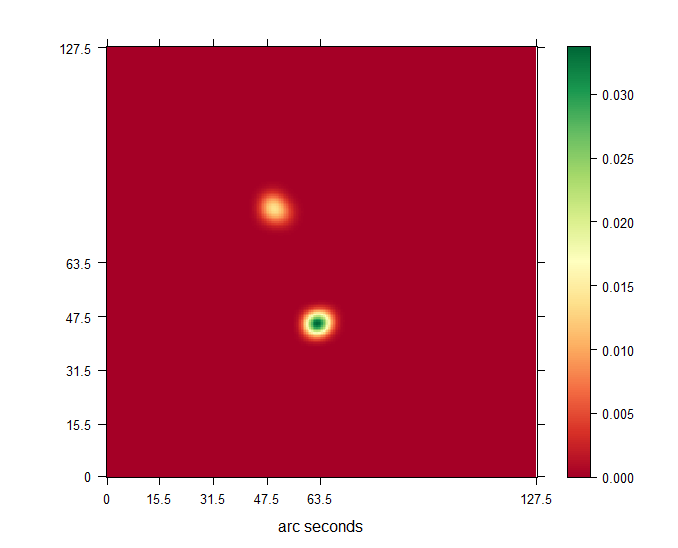
\includegraphics[width=\linewidth]{./chapters/20.results/points/cd.png}
		\caption{Coordinate Descent reconstruction.}
		\label{results:points:cd}
	\end{subfigure}
	
	\caption{Image reconstruction of two point sources.}
	\label{results:point}
\end{figure}

Both algorithms have free parameters to tune. tCLEAN has a several parameters, but, CASA's default values were used except for the maximum number of CLEAN iterations (parameter niter), which was set to 250. The proof-of-concept Coordinate Descent implementation has three parameters to tune: Number of iterations, the number of starlet layers $J$, and the regularization parameter $\lambda$. The first two parameter could be estimated by the reconstruction algorithm itself. For this implementation, it was left to the user. For the two simulations the Coordinate Descent parameters were chosen:
\begin{itemize}
	\item Two Point sources: 4 full iterations, $J=3$, $\lambda=0.1$
	\item Mixed sources: 4 full iterations, $J=7$, $\lambda=0.01$
\end{itemize}

In figure \ref{results:point} Coordinate Descent and tCLEAN reconstruction differ in two notable ways: The peak intensity of the source, and how much each algorithm spreads the point source. 

\textit{Spread:} tCLEAN essentially reconstructs a convolve version of the observed image. The observed image gets convolved with a Gaussian function, which represents the accuracy limit of the instrument. Coordinate Descent tries to reconstruct the observed image directly, resulting in a reconstruction where the sources are much less spread and completely separated. 

\textit{Intensity:} The reconstructions differ in intensity. The figure \ref{results:points:contour} shows the intensity profile of the two reconstructions. Note the $y$ axis is on a logarithmic scale. Also note that Coordinate Descent has shifted the smaller peak by a pixel in its reconstruction. [Total flux correct in CD?]

\begin{figure}[h]
	\centering
	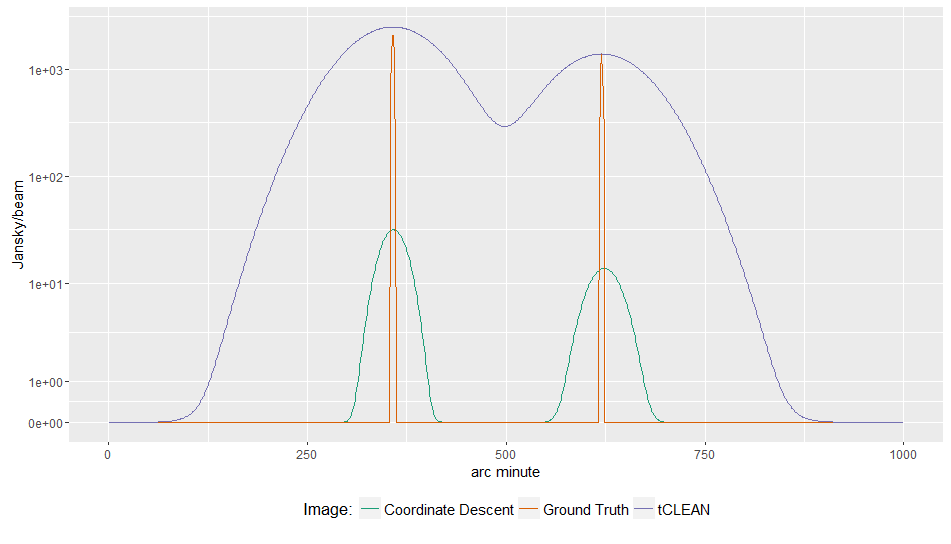
\includegraphics[width=0.8\linewidth]{./chapters/20.results/points/line.png}
	\caption{Intensity profile of the two point sources.}
	\label{results:points:contour}
\end{figure}

The difference in intensity becomes more apparent with extended emissions. Figure \ref{results:mixed} shows Coordinate Descent and tCLEAN on the simulation with mixed sources. Again the two reconstructions arrive at different intensities. The gaussian emissions are reconstructed with a higher intensity than Coordinate Descent.

\begin{figure}[h]
	\centering
	\begin{subfigure}[b]{0.4\linewidth}
		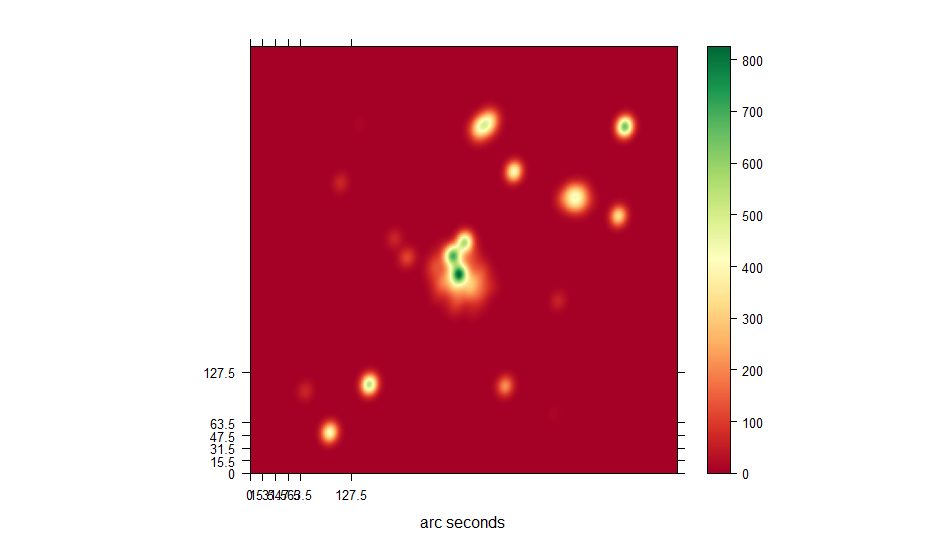
\includegraphics[width=\linewidth]{./chapters/20.results/mixed/mixed_tclean.png}
		\caption{tclean reconstruction}
		\label{results:mixed:tclean}
	\end{subfigure}
	\begin{subfigure}[b]{0.4\linewidth}
		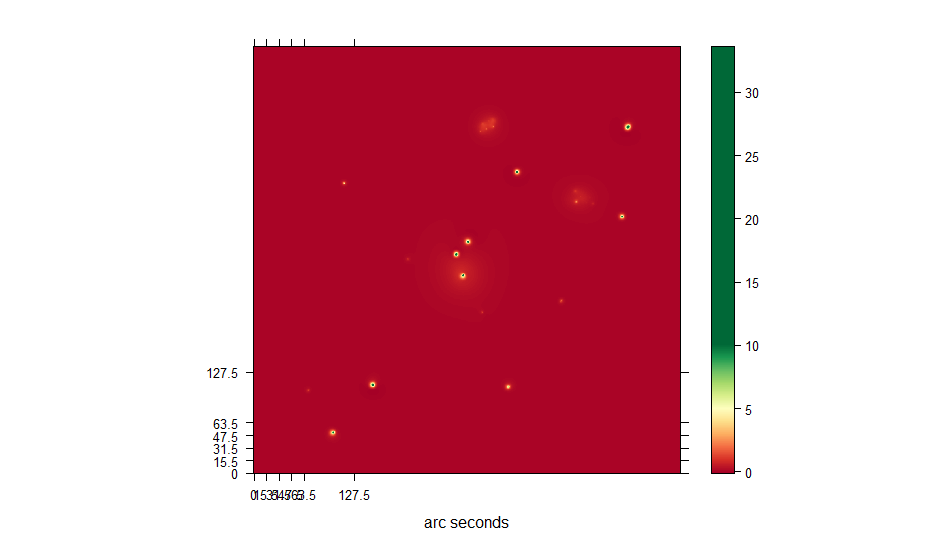
\includegraphics[width=\linewidth]{./chapters/20.results/mixed/mixed_cd.png}
		\caption{Coordinate Descent Reconstruction}
		\label{results:mixed:cd}
	\end{subfigure}
	\caption{Reconstruction on mixed sources}
	\label{results:mixed}
\end{figure}

With starlets, coordinate descent has a representation for extended emissions. Looking at the intensity profile of an extended emisions \ref{}, we see Coordiante Descent coming closer to the true intensity. Although in the four iterations,  [it still had a considerable margin on error]. 

Total flux constraint, $\lambda$ for different starlet layers like in \cite{girard2015sparse}

Coordinate Descent did not reconstruct all point sources. How many starlets are non-zero is the major point for runtime. It depends on how many areas of the image are non-zero. Starlet has a representation for extended emission, how many starlets are needed for modelling is hard.





\subsection{Scalability estimate of CLEAN and Coordinate Descent}
%\begin{figure}[h]
%	\centering
%	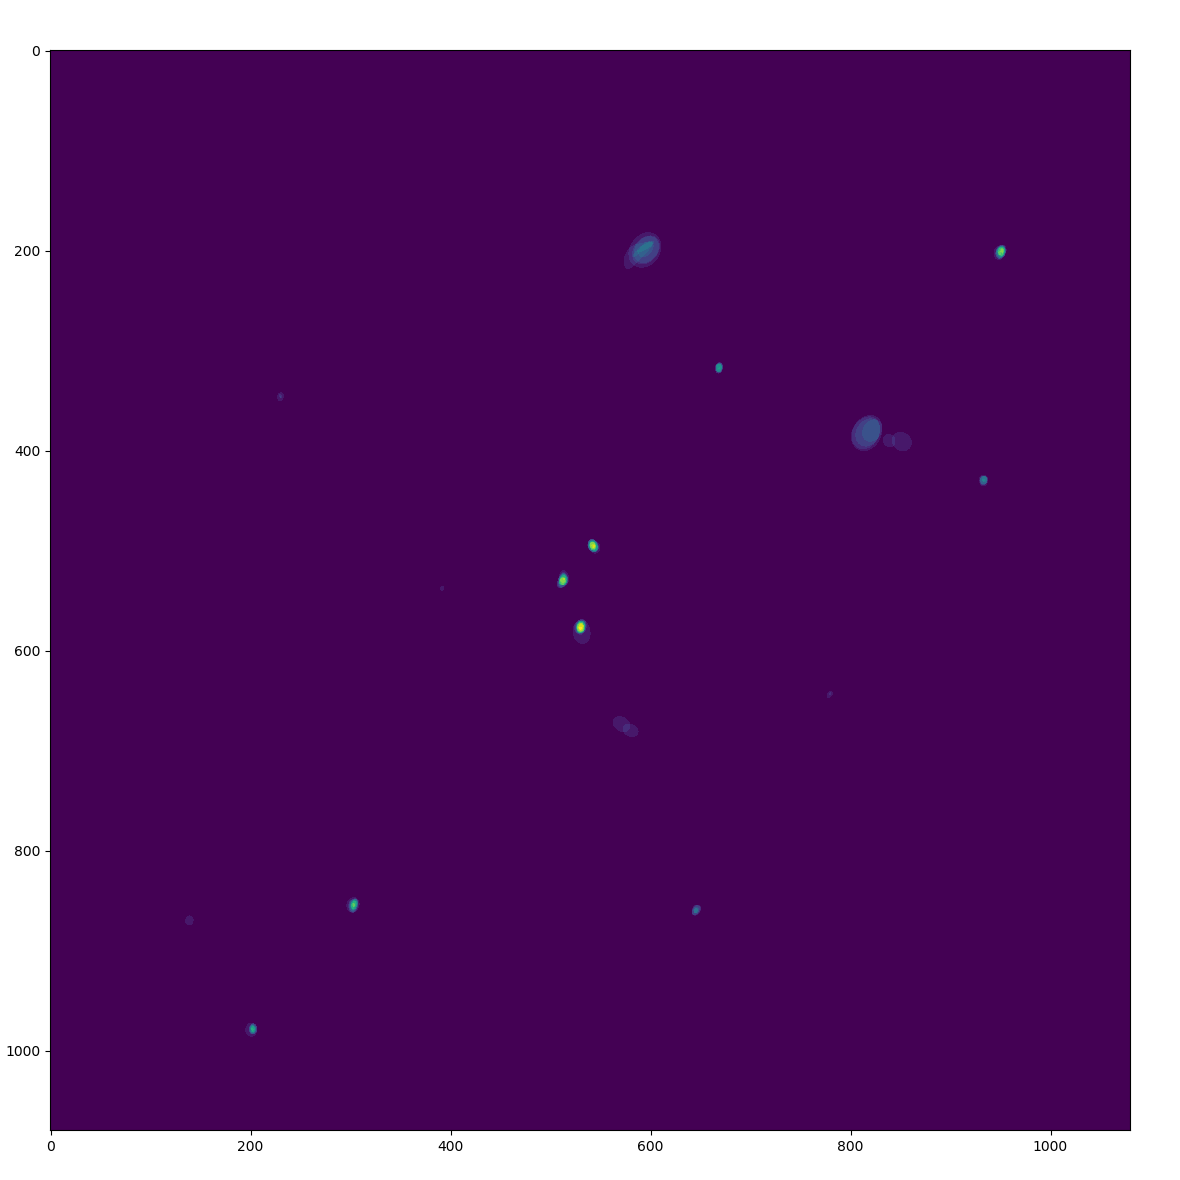
\includegraphics[width=0.5\linewidth]{./chapters/05.algorithms/sim00/full_cache_debug.png}
%	\caption{Pixels used to reconstruct the image}
%	\label{results:pixels:used}
%\end{figure}
Pinning down the precise runtime of Coordinate Descent is difficult. As mentioned in section \ref{cd}, Coordinate Descent has lose convergence guarantees in theory, but works well in practice with heuristics. However, these heuristics complicate the runtime analysis of Coordinate Descent. How well the active set heuristic performs on an average case is a difficult analysis.

Furthermore the current implementation can potentially be improved with other heuristics. In this section, we account for potential heuristics by looking at the best case runtime complexity of Coordinate Descent. We compare it to the complexity of CLEAN on a real MeerKAT observation. It turns out that CLEAN and the Major Cycle architecture eadd to a lower runtime complexity on large datasets.

\subsubsection{Runtime complexity of Coordinate Descent}
The runtime complexity of Coordinate Descent depends largely on the number of Visibilities $M$ and the number of non-zero starlets $S$. The number and location of the $S$ non-zero starlets are generally not known. However, we created a heuristic which finds likely non-zero starlet components. In a realistic setting, the heuristic will have found more than $S$ likely non-zero starlets. For the best case scenario, we assume an oracle performance heuristic: It finds the location and number of the $S$ non-zero starlet components in constant time ($O(1)$). Coordinate Descent therefore has to find the value of the $S$ non-zero starlet components, which takes three separate operations: creating the columns of $F^{-1}$, calculating the minima for each single component, and calculating the starlet layers:

\begin{alignat*}{1}
\text{creating} \:S\: \text{columns of}\: F^{-1} &: S*3M\\
\text{locating} \:S\: \text{minima of} \:S\: \text{parabolas} &: S*8M\\
\text{calculating} \:J\: \text{Starlet layers} &: J * 2M
\end{alignat*}

We assume we have enough memory to cache the columns of $F^{-1}$ and only need to calculate them once. Coordinate Descent arrives at the correct result in $I_{CD}$ iterations. Therefore we arrive at the runtime complexity of \eqref{results:cd:omega}.

\begin{equation}\label{results:cd:omega}
CD(I_{CD}, M, S, J) = S*3M + I_{CD} * [S * 8M + J * 2M]
\end{equation}

Note that the runtime of Coordinate Descent is independent of the number of pixels. The only image related parameter in \eqref{results:cd:omega} is $J$, the number of starlet layers. The largest starlet layer represents the largest possible structure in the image, which is given by the instrument and the image resolution (pixels per arc-second). The runtime only depends indirectly on the image resolution, not the total number of pixels.

Also note the term iterating over the $S$ non-zero starlets, $ I_{CD} * [S * 8M +\ldots]$. As it turns out, this is the Achilles heel of the algorithm. MeerKAT observations contain a very large amount of Visibilities $M$ and a large amount of distinct structures, which leads to a large $S$ (each point source needs at least one non-zero component to be represented). 

\subsubsection{Runtime complexity of CLEAN}
We look at CLEAN reconstructions which use the non-uniform FFT with $w$-stacking. The runtime of a single Major cycle depends on the non-uniform FFT with $w$-stacking and the number of CLEAN deconvolutions. The number $N$ denotes the number of pixels (for example $512^2$).

\begin{alignat*}{1}
	\text{non-uniform FFT} &: M + 2N*ld(2N)\\
	\text{non-uniform FFT with} \:w\text{-stacking} &:M + W*(2N*ld(2N) + 2N) + N*ld(N)\\
	I_{CLEAN}\: \text{deconvolutions} &: I_{CLEAN}*2N
\end{alignat*}

The overall complexity shown in \eqref{results:clean:o} can also be split into two parts: It depends on the number of Major on the number of Major Cycles $I_{Major}$ and the complexity of the non-uniform FFT, and $I_{Major}$ times the CLEAN deconvolutions. 

\begin{equation}\label{results:clean:o}
\begin{aligned}
 CLEAN(I_{Major}, I_{CLEAN}, M, N,  W) =\: &I_{Major} * 2 * [M + W*(2N log 2N + 2N) + N log N]\\
+ &I_{Major} * [I_{CLEAN}*2N]
\end{aligned}
\end{equation}

Notice that the number of CLEAN deconvolutions $I_{CLEAN}$ depends on the image content, similar the number of non-zero starlets $S$ for Coordinate Descent. Here however, it multiplies with the number of pixels $N$ instead of the number of Visibilities $M$. In a sense, the major cycle tries to reduce the runtime complexity of handling the image content by calculating the non-uniform FFT. If the difference is large enough $N \ll M$, then the Major Cycle will end up with a smaller overall runtime.

\subsubsection{Runtime complexity estimate on MeerKAT data}
The MeerKAT observation contains approximately 540 channels with 4 million calibrated Visibilities each. After calibration, MeerKAT data is typically averaged over frequency and time to reduce its disk space. There are no strict rules on how to chose the image resolution and number of pixels. An initial CLEAN reconstruction was preformed with an image size of $8192^2$ and 1.6 arc-seconds per pixel resolution. These numbers were used for the estimate.

Rest of the 



Example reconstruction was used, with image size ofpixels. The image size can vary between 

The image size is typically left to the user, and can vary widely. For this estimate, we use the $8192^2$ pixels as given


Complex formula. But for MeerKAT, the number of Visibilities $M$ is by far the largest. Simplifies to $M_{Major}*M$

Assumptions
Estimates for $M_{Major}$ = 10. (Cite New W-stacking approach)
W = $100$ depends on observation between 10, and hundreds. Depends on the observation. Cite new w-stacking approach can limit the number of w-stacks. 
D=35'000

Assumptions for $J$ = 10


In terms of $S$ for 
Where the data comes from

Calibration: 
Visibilities = 4060770
Channels = 540

pixels = 8192 * 8192 = 67 108 864

Target, what would an Ideal Compressed Sensing implementation do.

Memory requirement

MeerKAT has by far more Visibilities than pixels

Write one meerkat observation

\begin{figure}[h]
	\centering
	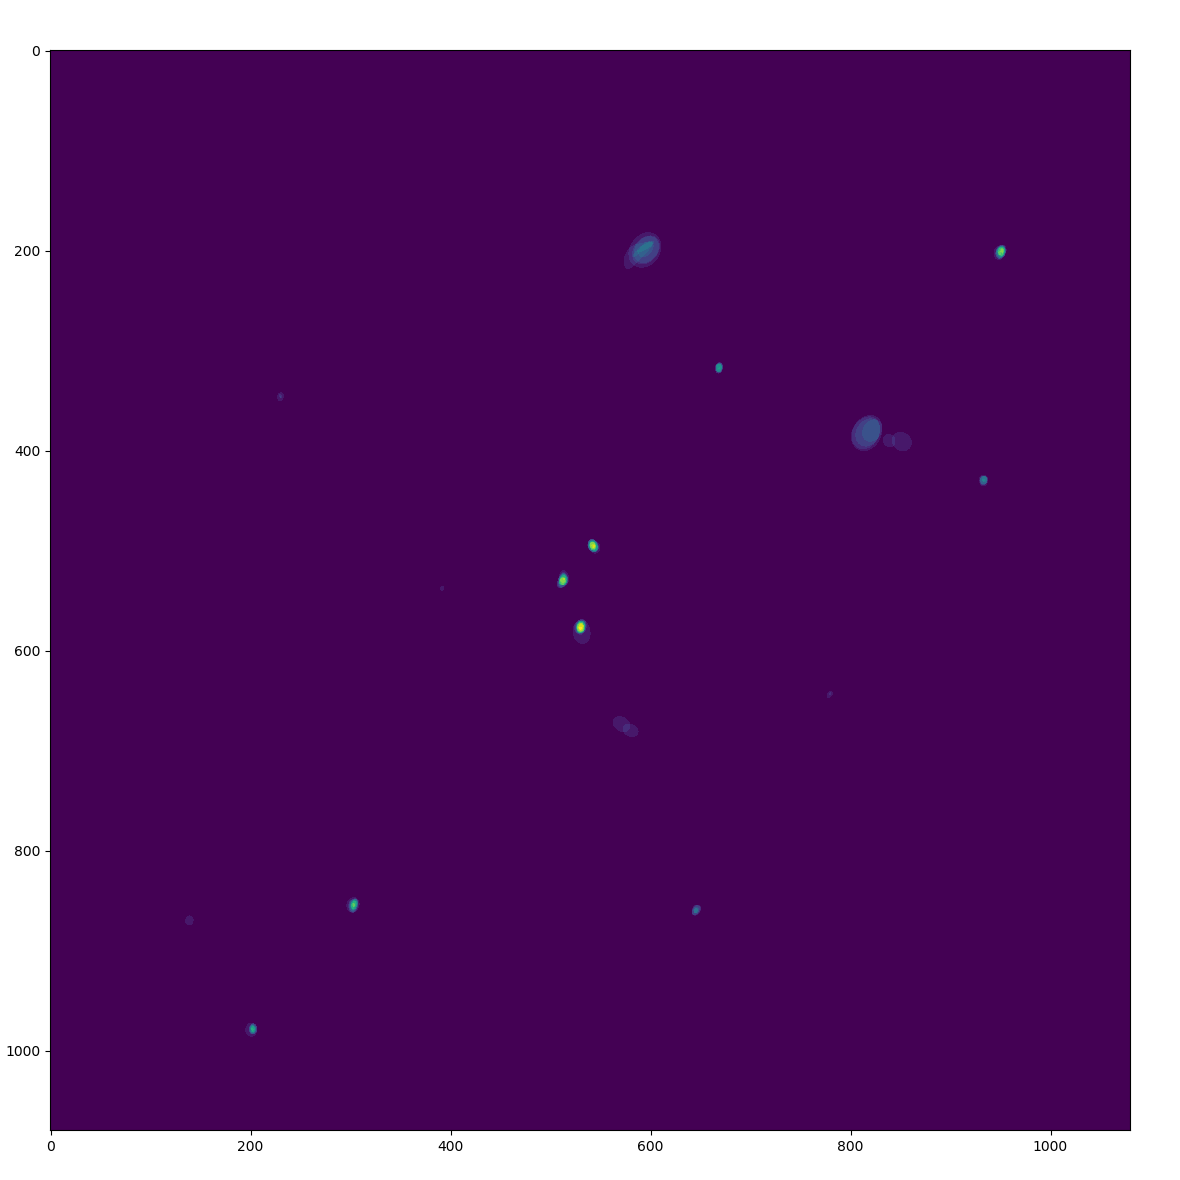
\includegraphics[width=0.5\linewidth]{./chapters/05.algorithms/sim00/full_cache_debug.png}
	\caption{WSCLEAN Reconstruction of a MeerKAT observation.}
	\label{results:wsclean}
\end{figure}
The number of $S$ and then the lower bound of Coordinate Descent. (Put WSCLEAN image in here and Discuss $S$)



Other compressed sensing approaches have a more expensive term than $D*2N$ for their complexity. But compared to compressed sensin.


IMAGE CONTENT SCALES WITH pixels instead of Visibilities.

